
\section{Sicherheitsmaßnahmen}
Um die Sicherheit während der Benützung des Luftkissenboots zu gewährleisten wurden mehrere Sicherheitsvorkehrungen getroffen.
\subsection{Not-Aus-Schalter mit Schlüssel}
Die Notabschaltung der Regler, und damit auch der Motoren, erfolgt durch Betätigen des Not-Aus-Schalters, da dies den Haltestrom des Hauptrelais unterbricht. 
Es ist möglich das Hovercraft nach einer Notabschaltung mit Hilfe des Schlüssels wieder zu starten. 

\begin{figure}[h]
    \centering
    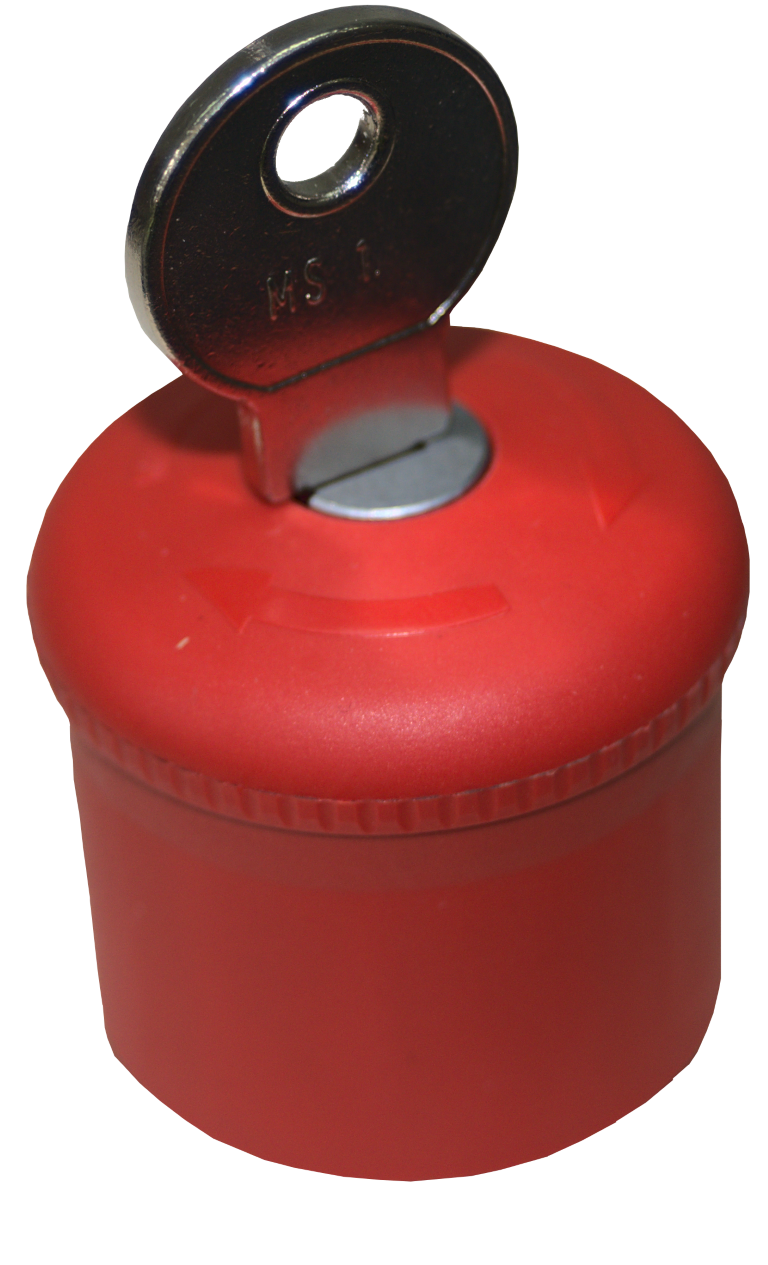
\includegraphics[width=0.25\textwidth]{Fotos/Notaus.png}
    \captionof{figure}{Notausschlüsselschalter}    
\end{figure}
  
\newpage
\subsection{Daumengas für beide Propeller}
Durch Betätigen der beiden Daumengase, rechts und links am Lenker, erfolgt der Antrieb der Propeller. Das linke Daumengas ist für den Auftrieb, für den unteren Propeller und
das rechte für den Antrieb, den hinteren Propeller. Durch Loslassen des Daumengases bremst das Hovercraft sofort.

\begin{figure}[h]
    \centering
    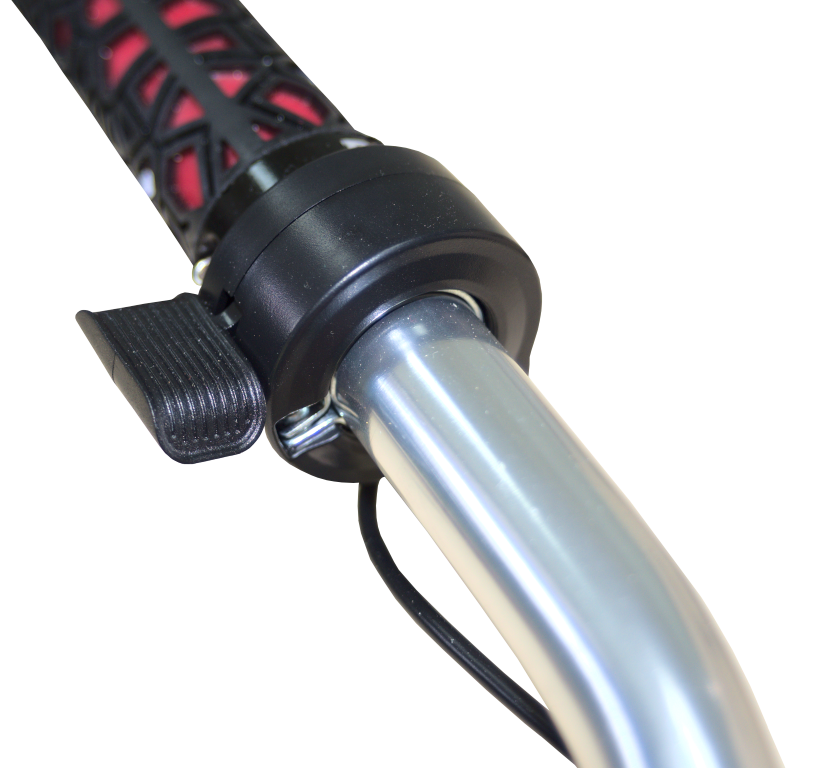
\includegraphics[width=0.5\textwidth]{Fotos/Daumengas.png}
    \captionof{figure}{Daumengas}    
\end{figure}


\subsection{Gitterabdeckungen}
Über den beiden Propellern befinden sich Gitter, die es unmöglich machen, bewusst oder unbewusst in ein drehendes Teil zu fassen. 
Weiters dienen die Gitter als Schutz vor losen Teilen, die sich in den Propellern verfangen könnten. 

\begin{minipage}{13cm}
    \centering
    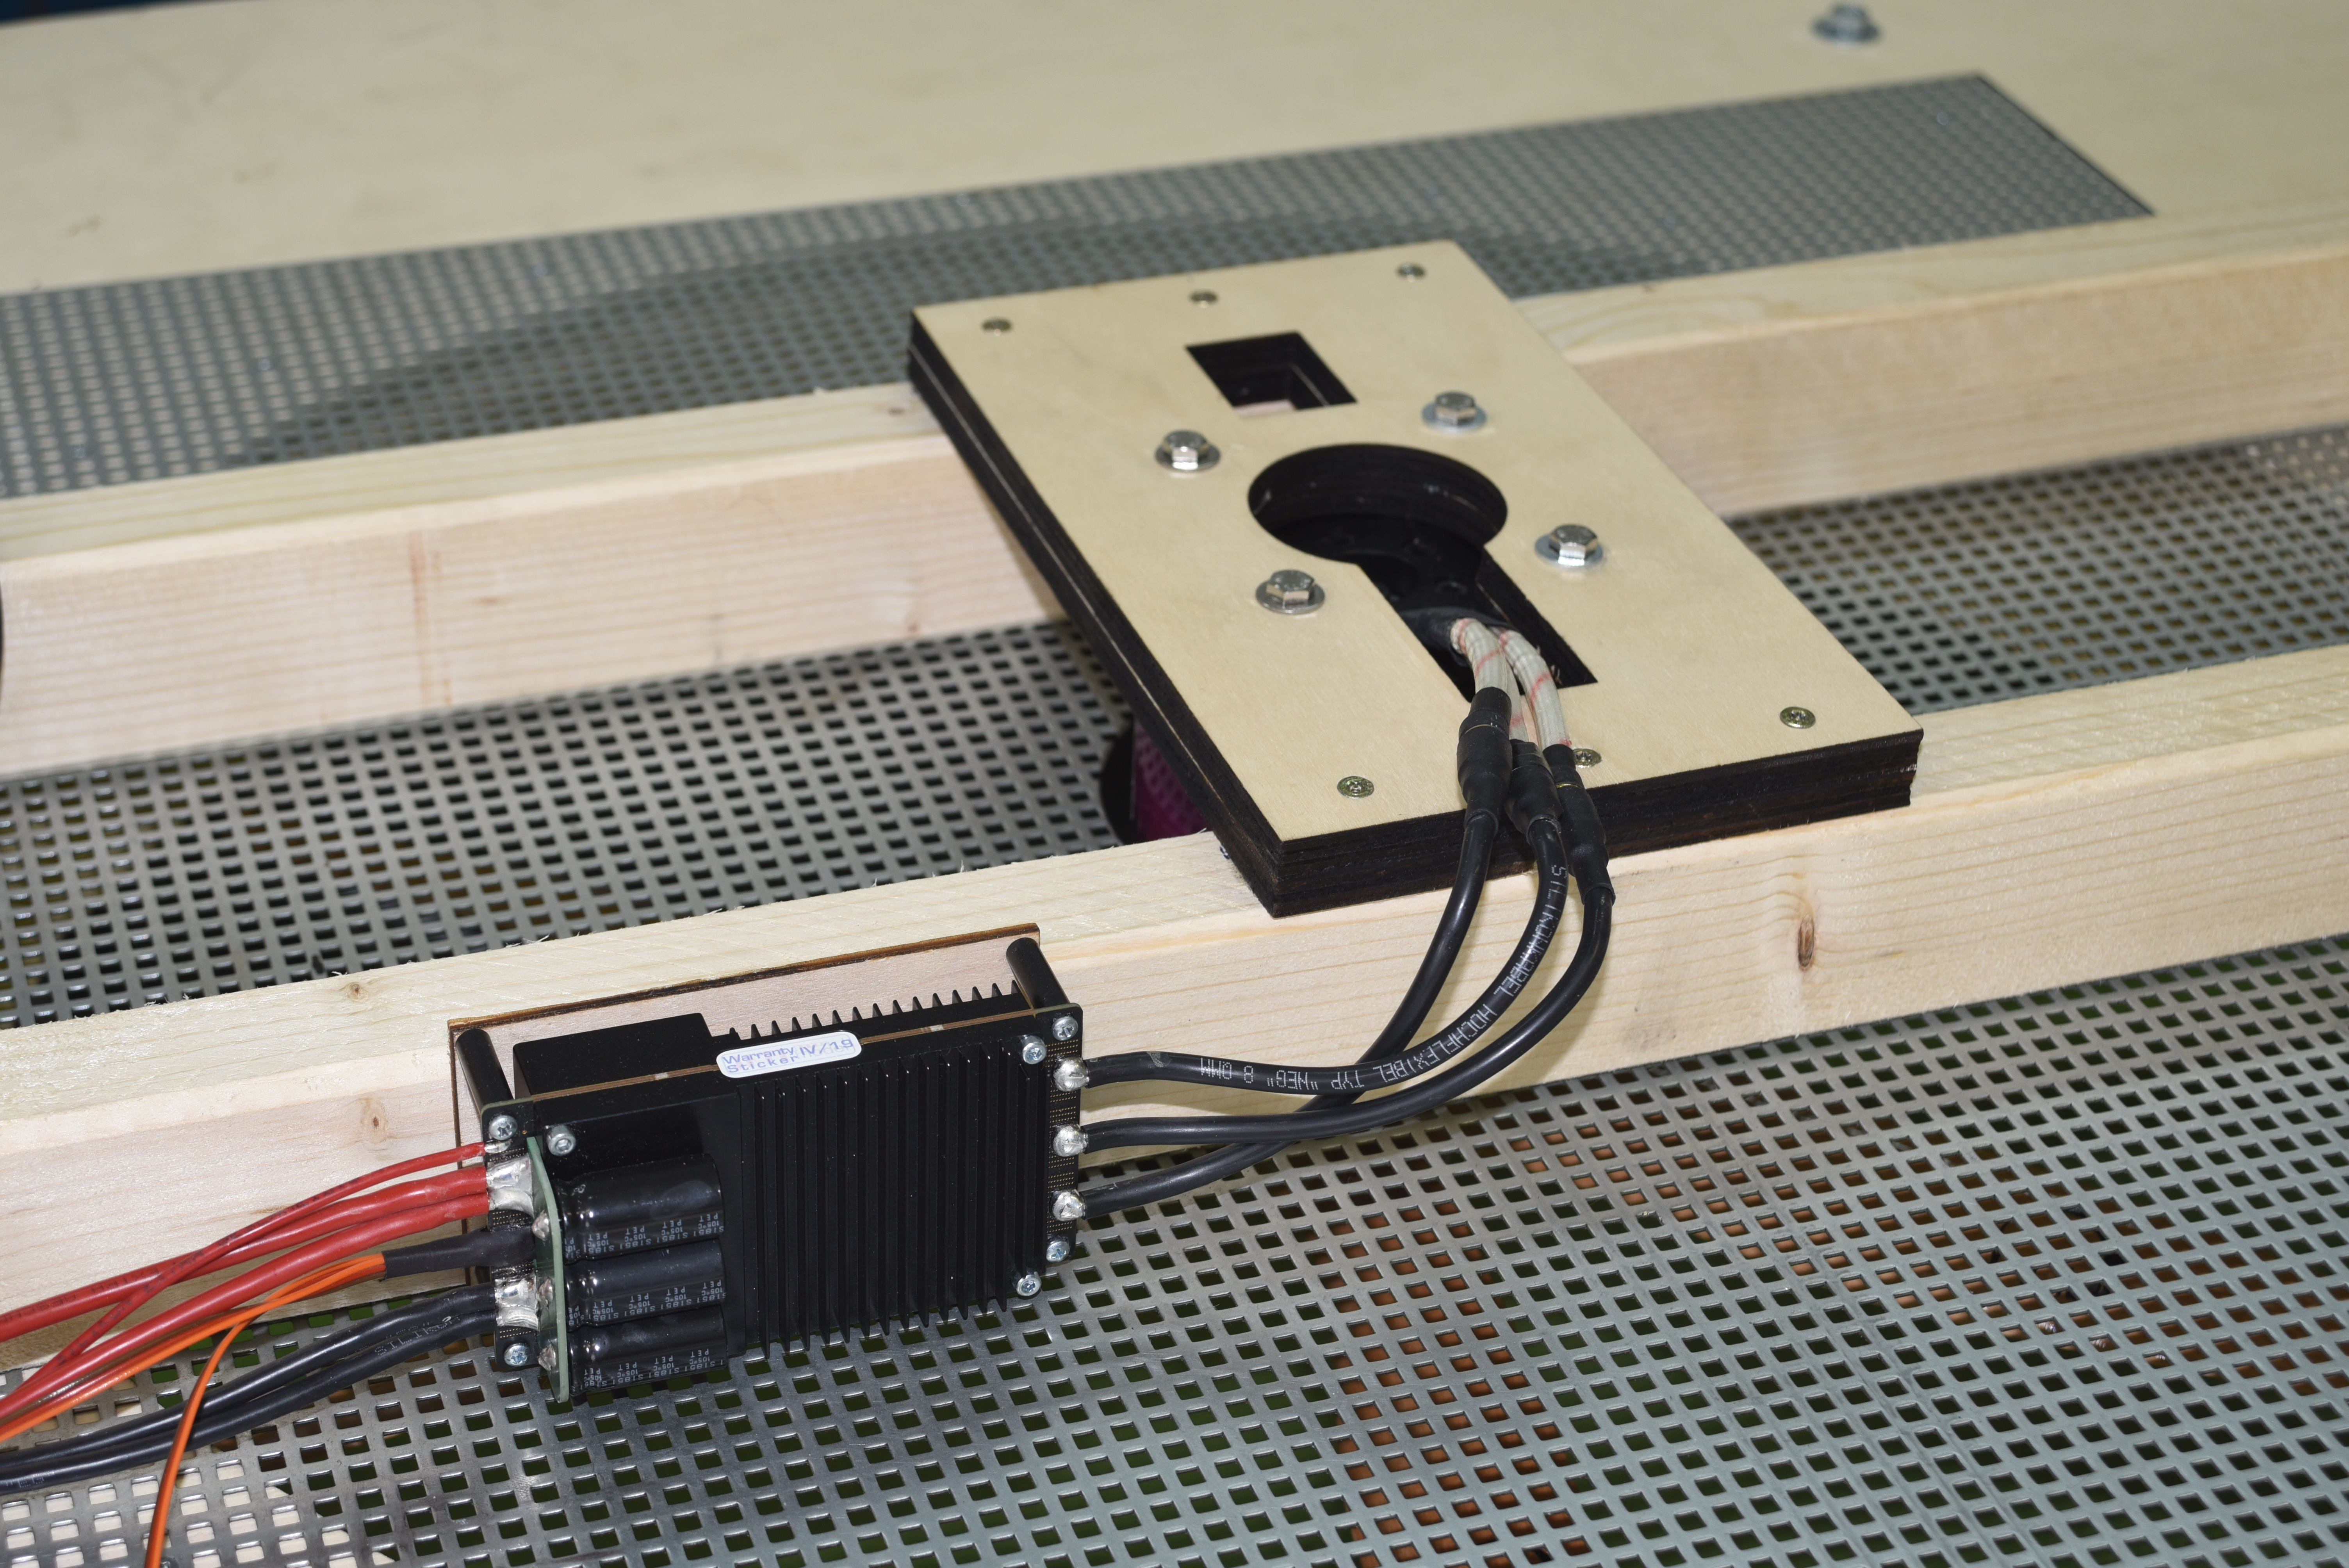
\includegraphics[width=0.5\textwidth]{Fotos/Gitter_unten.jpg}
    \captionof{figure}{Unteres Gitter}   
\end{minipage}

\todo[]{Gitter hinten}
\section{Gerätesicherheit}

\subsection{Not-Aus gedrückt \& Ladedeckel offen bei Ladevorgang}
Während dem Ladevorgang ist es notwendig, den Not-Aus betätigt zu haben, siehe \ref{sec:Anleitung_Laden} um eine sichere Trennung vom Relais zu bieten. \\
Weiters ist es notwendig, den Ladedeckel zu öffnen. Dies wird mithilfe von Schaltern überprüft. Falls der Ladedeckel offen ist, lässt sich das Hovercraft nicht starten.

\subsection{Bremsschutz}
Zum Schutz des Schlauchbootbodens beim Bremsen wurde ein zusätzlicher Boden angebracht. Dieser wurde mit einem Kraftkleber und Lochband am Boot befestigt. 
Der zusätzliche Boden bietet Schutz vor Steinen und ähnlichem, was das Boot zerstören könnte. 

\begin{figure}[h]
    \centering
    \includegraphics[width=0.5\textwidth]{Fotos/Konstruktion/DSC_8616.png}
    \captionof{figure}{Bremsschutz}    
\end{figure}


\subsection{Regler Kühlung}
Die beiden Motorregler sind so positioniert, dass sie luftgekühlt und vor dem Überhitzen geschützt sind. Weiters haben sie auch eine automatische Abschaltung bei Übertemperatur
eingebaut. Diese wurde auf $90^\circ C$ eingestellt. 

\subsection{KFZ-Sicherungen}
Die KFZ-Sicherungen der Firma SIBA wurden eingebaut um die Akkus vor einem Kurzschluss zu schützen. Die KFZ-Sicherung haben einen Nennstrom $I_\mathrm{n} = 500\mathrm{A}$
und eine Nennspannung $U_\mathrm{n} = 60 \mathrm{V}$.